\documentclass[SoftwareDesign/SoftwareDesign_main.tex]{subfiles}
\begin{document}
\section{Design af User Sign up}
I dette afsnit præsenteres designet af den, hvor en bruger, der ønsker at registrere sig som bruger på applikationen, kan registrere sig. Dette afsnit beskriver både design af udseendet på siden, samt design af funtkionaliteten af siden og databehandling af bruger inputs.
\subsection{Design af View til user sign up}
Som de andre views tager designet udgangspunkt i en udarbejdet WireFrame, der kan ses i figur \ref{fig:signup_wf}.
\begin{figure}[H]
    \centering
    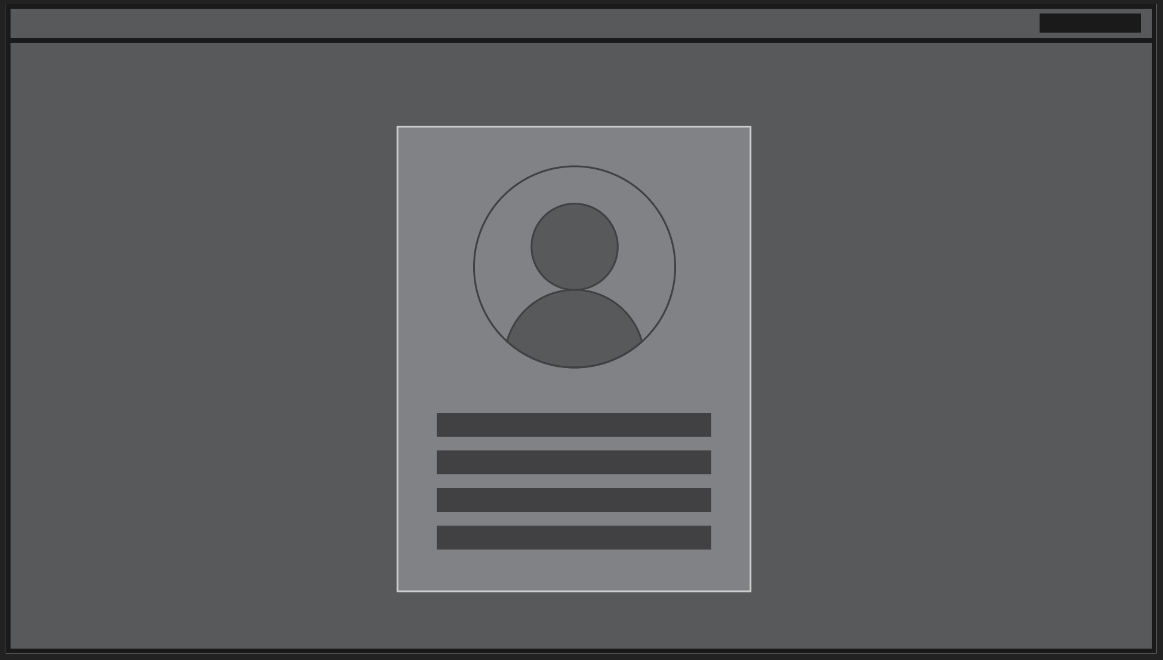
\includegraphics[width=\textwidth]{SoftwareDesign/MVVMDesigns/Graphics/SignupWireFrame.png}
    \caption{WireFrame for Sign Up view}
    \label{fig:signup_wf}
\end{figure}
WireFramen i figur \ref{fig:signup_wf} beskriver det overordnede layout på siden, men også lidt funktionalitet i forhold navigation, hvilket dog kræver den fulde WireFrame. Dog kan det af denne ses, at der skal kunne navigeres mellem Login- og Signup-siderne. Da der på denne side kommer til at være meget bruger input, så bliver der også nødt til at være en form for indikation til brugeren, hvis de indtastede data ikke er valide. Dette kan dog umiddelbart løses ved at ændrer på stylingen af text-inputs til at vise dette på en pæn måde.
\subsection{Design af ViewModel til user sign up}
Denne ViewModel kommer i store træk til at bære præg af \textbf{Security View} fra arkitekturen, da der her håndteres brugerinformation og sensibel data, som brugerens koderord. Derfor bestræbes der efter ikke at holde nogle kodeord i clear-text i hukommelse (Variable eller lignende), men samtidig opnå den MVVM struktur, der ønskes i applikationen. Dette kræver dog et kompromis på sikkerhed, da der skal tilgås C\# Passwordboxes via en monitor der hooker sig ind via en attached property. Dette er dog nødvendigt for at få fat i kodeordet i et SecureString format. Da der ikke kan sendes SecureString passwords til databasen, laves en SecureString hjælpe klasse, der kan konvertere SecureString til en string. Denne hjælpeklasse kan anvendes sammen med to PasswordBoxes for at lave en klassisk validering af brugerens kodeord er det brugeren egentlig ønsker. Til der udarbejdes et IValidator-interface, med en Validate funktion . Til interfacet tilføjes en PasswordValidator, der validerer om brugerens kodeord er mere end 6 karakterer langt og indeholder både tal og karakterer. Dette pådutter brugeren en form for sikkerhed omkring deres bruger, hvilket er i overensstemmelse med \textbf{Securit View}. Desuden laves der også en validator, der validerer om den indtastede email er en valid email.

\end{document}